\documentclass[a4paper,oneside]{book}

\usepackage{dolgozat}

\usepackage{listings}
\usepackage{tikz}

\usepackage{rotating}

\usepackage{color}
\usepackage{soulutf8}
% \definecolor{comment}{rgb}{0,0.6,0.2}

\usepackage{CJKutf8}
\usepackage{graphicx}
\usepackage[utf8]{inputenc}
\usepackage{hyperref}
\usepackage{marginnote}
\usepackage{listings}
\graphicspath{ {../dolgozat/images/} }


% Code colorature
\definecolor{paszt}{RGB}{252,252,252}
\definecolor{keret}{RGB}{220,220,220}
\lstset{
backgroundcolor=\color{paszt},
% showlines=true,
framexleftmargin=4mm,
framexrightmargin=4mm,
framextopmargin=2mm,
framexbottommargin=2mm,
frameround=tttt,
frame=trbl,
rulecolor=\color{keret},
extendedchars=true,
literate={á}{{\'a}}1 {é}{{\'e}}1 {ö}{{\"o}}1 {ő}{{\H{o}}}1 {ó}{{\'o}}1,
%inputencoding=utf8
}

% Line spacing (1.5-ös sorköz)
\linespread{1.2}

% Set spacing in source code (normál sorköz -1.5)
%\lstset{
%lineskip={-3pt}
%}

\usepackage{pslatex}

%%% Font settings
% \usepackage{times}
\usepackage{lmodern} % !!!
% \usepackage{chancery}
% \usepackage{charter}
% \usepackage{palatino}
% \usepackage{mathpazo}
% \usepackage{mathpple} % !!!
% \usepackage{mathptmx}

\usepackage{pstricks}

\usepackage{cpp}
\usepackage{python}

% Indicators
\usepackage{indicators}

\begin{document}

% \pagestyle{empty} %a címlapon ne legyen semmi=empty, azaz nincs fejléc és lábléc

% Címlap
\pagestyle{empty} %a címlapon ne legyen semmi=empty, azaz nincs fejléc és lábléc

\begin{flushleft}
\textsc{\bfseries Miskolci Egyetem}\\
Gépészmérnöki és Informatikai Kar\\
Általános Informatikai Intézeti Tanszék
\end{flushleft}

%A fõiskola logoja
{\large
\begin{center}
\vglue 1truecm
\textbf{\huge\textsc{Szakdolgozat}}\\
\vglue 1truecm

\epsfig{file=images/ME_logo.eps, width=4.8truecm, height=4truecm}\\
\textbf{\textsc{Miskolci Egyetem}}
\end{center}}

\vglue 1.5truecm %függõleges helykihagyás

%A szakdolgozat címe, akár több sorban is
{\LARGE
\begin{center}
\textbf{Kínai karakterek felismerése konvolúciós neurális hálók használatával}
\end{center}}

\vspace*{2.5truecm}
%A hallgató neve, évfolyam, szak(ok), a konzulens(ek) neve
{\large
\begin{center}
\begin{tabular}{c}
\textbf{Készítette:}\\
Szilvási Péter\\
Mérnökinformatikus BSc
\end{tabular}
\end{center}
\begin{center}
\begin{tabular}{c}
\textbf{Témavezető:}\\
Piller Imre, egyetemi tanársegéd
\end{tabular}
\end{center}}
\vfill
%Keltezés: Hely és év
{\large
\begin{center}
\textbf{\textsc{Miskolc, 2018}}
\end{center}}

\newpage


% Font size
% \large

% Tartalomjegyzék
\tableofcontents
\thispagestyle{empty}
\cleardoublepage

% Set page style !!!
\pagestyle{fancy}

% Set number of page
\setcounter{page}{1}

% Chapters
\Chapter{Bevezetés}

% TODO: Feature extraction-t, tesztelést, validálási módokat érdemes hangsúlyozni majd.

\Chapter{Kínai karakterek felismerése}

\section{Az alapvonások}

Az írásjegyek megrajzolásának az egyik elsődleges szabályát az írásjegy vonásainak sorrendje adja \cite{kinaiiras}. Az írásjegyek -- bármilyen bonyolult legyen is némelyik -- tulajdonképpen néhány igen egyszerű vonalból épülnek fel. Ezek az írásjegyek alapelemei, vagy alap-ecsetvonásai. \Aref{fig:alapvonasok}. ábrán az alapvonások néhány főbb típusa látható. Természetesen az alapvonásoknak több változata is lehetséges (méret, vastagság, irány) attól függően, hogy az írásjegy melyik részén helyezkedik el.

\begin{figure}[h]
	\centering
	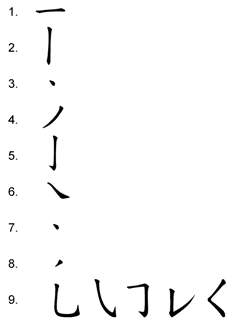
\includegraphics[scale=0.5]{chinese_strokes}
	\caption{A kínai karakterek alapvonásai}
	\label{fig:alapvonasok}
\end{figure}

Minden egyes vonásnak megvan a felépítési szabálya: az ecsetvonásoknak meghatározott sorrendben kell követniük egymást, még pedig általános elvként az írásjegyek határait alkotó virtuális négyszög bal felső sarkából lefelé és jobbra haladva. Az írásjegy gerincét, fő szerkezeti elemét adó nagyobb vonást, ha az egész írásjegyet átjárja, legutoljára húzzák.

\section{A vonássorrend szabályai}

Az előző szakaszban említett általános elv mellett az alábbi szabályokat alkalmazhatjuk az írásjegyek vonásainak sorrendjének meghatározásához.
\begin{enumerate}
	\item A vízszintes vonások megelőzik a függőleges vonásokat.
	\item A balra lejtő vonások megelőzik a jobbra lejtő vonásokat. 
	\item Az írásjegyek írását felülről kell kezdeni. 
	\item Az írásjegyet balról jobbra haladva építik fel. 
	\item A felülről keretezett írásjegyeknél előbb a keretet kell meghúzni. 
	\item Az alulról keretezett írásjegyeknél a keretet legvégül kell meghúzni. 
	\item A teljes keretet mindig legvégül kell bezárni.
\end{enumerate}

Egy szimmetrikus felépítésű írásjegynél előbb a középső részt kell kialakítani, s csak azután az oldalakat. Erre láthatunk egy példát \aref{fig:sorrend_pelda}. ábrán.

\begin{figure}[h]
	\centering
	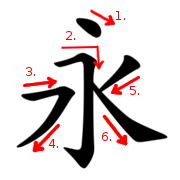
\includegraphics[scale=1.0]{images/vonasrend_ordered.png}
	\caption{Példa egy szimmetrikus írásjel vonásainak sorrendjére}
	\label{fig:sorrend_pelda}
\end{figure}

A kínai írásjegyek különböző számú alapvonásokból épülhetnek fel. Ezek közül a legegyszerűbb a csupán egyetlen vízszintes vonalból álló „egy” jelentésű \begin{CJK*}{UTF8}{gbsn}
一
\end{CJK*} ji írásjegy. A kínai írásrendszer más, egy vonásból álló írásjegyet nem tartalmaz. Aránylag ritkák a két vonásból álló írásjegyek is, például: \begin{CJK*}{UTF8}{gbsn}
二
\end{CJK*} er„kettő”,
\begin{CJK*}{UTF8}{gbsn}
十
\end{CJK*} si „tíz”,
\begin{CJK*}{UTF8}{gbsn}
人
\end{CJK*} zsen „ember” stb. A hagyományos írásjegyek zöme 15–30 vonásból épül fel (átlagosan 9 vonásból). Esetenként azonban ennél jóval több vonásból álló írásjegyek is előfordulhatnak, melyek tulajdonképpen már több önálló írásjegy összevonásának is tekinthetők. Ritkák ugyan, de léteznek 50 vagy akár 80 vonásból álló írásjegyek is.\Aref{fig:char_numbers} ábrán láthatjuk a karakterek mennyiségét stroke-ok száma szerint.

\begin{figure}[h]
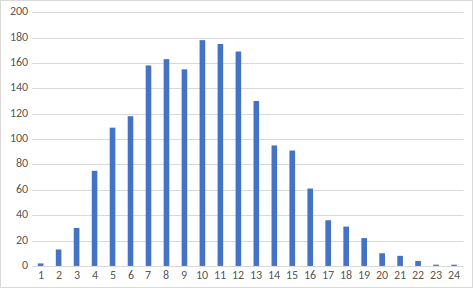
\includegraphics[scale=0.85]{images/chinese_char_by_strokes}
\centering
\caption{Kínai karakterek száma stroke-ok szerint}
\label{fig:char_numbers}
\end{figure}

\section{OCR megvalósítások}

\subsection{Az optikai karakterfelismerés feladata}

A különböző formátumú dokumentumok kezelésének egyik speciális esete, amikor a kezelendő dokumentumok még nem állnak rendelkezésre elektronikus formában. Ebben az esetben szinte mindig arról van szó, hogy a dokumentumok kinyomtatva, papír alapú hordozón jelennek meg. A későbbi feldolgozáshoz értelemszerűen digitalizálni kell a még nem digitalizált, papíron, nyomtatásban vagy írásban meglévő dokumentumokat, hogy az után elektronikusan szerkeszthető és feldolgozható legyen. Ebben a szituációban kap szerepet az optikai karakterfelismerés (\textit{Optical Character Recognition}, OCR). Az optikai karakterfelismerés a mesterséges intelligencia jelfeldolgozó és generalizációs képességeit kiaknázva képes nyomtatott, papír alapú dokumentumokon lévő karaktereket felismerni \cite{liu2013online}.

Az alap probléma itt az, hogy a nyomtatott, papír alapú dokumentumok esetében nagy zajaránnyal kell megküzdeni annak érdekében, hogy a releváns információt kinyerjük az érzékelt képi jelek és minták közül. Nyomtatott dokumentum esetében ilyen zajnak tekinthető például egy apró folt a papíron, tintaelmosódás, tintahiány, homályos háttér, apró gyűrődés a papíron, túl közeli vagy egybeolvadó betűk, betű dőlésszögének ingadozása stb. Kézírás esetén a kihívás még nagyobb, hiszen itt a személyiségjegyek sokszínűségéből adódó írásminták kavalkádjából kell megküzdeni, hogy fel tudjuk imsertetni a karaktereket. Mind a nyomtatott, mind pedig a kézírásos esetben az optikai karakterfelismerő rendszer egy tanulási fázist követően képes olyan mintákat is osztályozni (a megfelelő karaktert felismerni), amelyekkel a tanulási fázisban nem találkozott, tehát megvan a szükséges generalizációs képessége.

Vannak készen elérhető OCR megoldások \cite{tmwebdvi77}, amelyek tipikusan az alábbi két részből állnak.
\begin{enumerate}
\item A szkennelő fejből, amely a dokumentum egészét vagy részeit beszkenneli. Hardverről van szó, ami elvégezi a digitalizálást. Két fizikai jelenségen alapszik fényvisszaverődésen és a fényelnyelésen.
\item  A mesterséges intelligencia szoftverből, ami elvégezi a beérkezett minták osztályozását, azaz magát a karakterfelismerést.
\end{enumerate}

\begin{figure}[h]
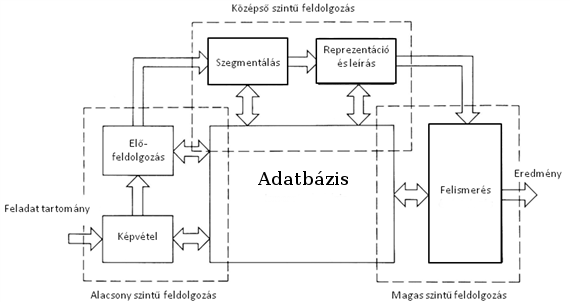
\includegraphics[scale=0.65]{images/ocr}
\centering
\caption{Az OCR-es feldolgozás szintjei}
\label{fig:feldolgozasi_szintek}
\end{figure}

Az OCR-el való feldolgozás során alapvetően három szintet \cite{feldolgozasi_szintek} különböztethetünk meg (\ref{fig:feldolgozasi_szintek}. ábra). 

\begin{enumerate}
\item Alacsony szintű (\textit{low-level}) feldolgozás
	\begin{itemize}
	\item A bemenet egy zajos kép, a kimenet pedig már egy tisztított, későbbi feldolgozásra alkalmasabb kép.
	\item Itt a kép minőségének a javításához az elterjedt képfeldolgozási előfeldolgozó algoritmusokat használják.
	\item Jellemző előfeldolgozások: \textit{zajszűrés, élesítés, finomítás, világosítás, maszkolás}.
	\end{itemize}
\item Középső szintű (\textit{intermediate-level}) feldolgozás
	\begin{itemize}
	\item A bemenetek képek, de a kiementek már a képekből nyert jellemzők.
	\item A kép komponenseinek kiemelése (szegmentálás) és azok jellemzése.
	\item Bizonyos mértékű mesterséges intelligencia/gépi tanulás szükséges lehet hozzá.
	\end{itemize}
\item Magas szintű (\textit{high-level}) feldolgozás
	\begin{itemize}
	\item A felismert objektumok együttesének érzékelése (osztályozási probléma).
	\item Felismerés és értelmezés (interpretáció).
	\item Ezen a szinten kap kiemelt szerepet a mesterséges intelligencia módszereinek alkalmazása.
	\end{itemize}
\end{enumerate}

Az adatok kezelését struktúrált, ellenőrzött formában érdemes megoldani, amihez ilyen esetben adatbázis szükséges. Az adatbázisban alapvetően az alábbi adatokat tárolhatjuk.

\begin{itemize}
\item A felismerni kivánt képek halmaza. 
\item A képekhez tartozó címkék, annotációk, amelyek szükségesek a mesterséges intelligencia tanítása során.
\item Különféle paraméterezések, konfigurációval kapcsolatos adatok.
\end{itemize}

Az interneten rengeteg adatbázis található: \textit{mnist, imagenet, kaggle, CASIA}.

\subsection{Szegmentációs módszerek}

A szegmentáció során a karakterek közötti éles határ megtalálása a cél annak érdekében, hogy téves minták ne kerüljenek osztályozásra (például két fél karakter). A szegmentáció feladata lehet az is, hogy a karakter-dőlésszögeket, karakterméreteket normalizálja. Sok esetben a szöveges dokumentumokban nem csak karakterek vannak, hanem képek és egyéb, a felismerés szempontjából nem lényeges szimbólumok. A szegmentáció további feladata tehát az is, hogy az ilyen, számunkra nem releváns grafikus objektumok közül kiszűrje a csak karaktereket tartalmazó szöveges részeket. \Aref{fig:ocr_segmentation}. ábrán láthatunk egy példát arra, hogy hogyan képes az algoritmus kiemelni az egy karakterhez tartozó képrészt.

\begin{figure}[h]
\centering
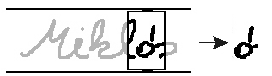
\includegraphics[scale=1.0]{images/ocr_segmentation}
\caption{Példa egy név karaktereinek a szegmentálására (forrás: \cite{tmwebdvi77})}
\label{fig:ocr_segmentation}
\end{figure}

\subsection{Optikai előfeldolgozás}

Az előfeldolgozás a bemeneti minta komplexitásának csökkentésére szolgál, és annak legjellemzőbb vonásait emeli ki. Különösen nagy jelentősége van a kézírás felismerésekor, ugyanis az írott betűk jóval komplexebb mintákat alkothatnak, mint a nyomtatott betűk. A jellemzők kiemelése során a komplexitás úgy csökken, hogy közben a legjellemzőbb információk megmaradnak és ezáltal a későbbi feldolgozás számításigényét redukálhatjuk. Ez a folyamat tulajdonképpen egy komplexitáscsökkentéssel járó digitalizáció. \Aref{fig:ocr_preprocess}. ábra egy egyszerű digitalizálási módszert mutat, amikor az analóg jelre egy mátrixot reprezentáló rácshálót illesztünk, és amelyik cellán átmegy az analóg karakter, az az elem a mátrixban 1 értéket vesz fel (fekete), egyéb esetben pedig 0-t (fehér). (Természetesen konvenciótól függően fordított eset is elképzelhető.)

\begin{figure}[h]
\centering
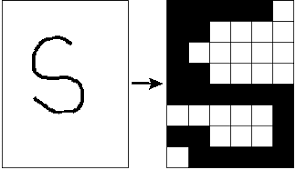
\includegraphics[scale=0.65]{images/ocr_preprocess}
\caption{Jellemzők kinyerésének egy fázisa, amely a dimenzió csökkenésével jár}
\label{fig:ocr_preprocess}
\end{figure}

\subsubsection{Dimenzió csökkentés}

A dimenziószám csökkentése optimálizálási folyamatnak tekinthető. A kivont jellemzőkben található redundáns információkat távolítja el. A tipikus dimenzió redukciós algoritmusok a gépi tanulás terén két részre oszthatók \cite{zhang2009patch}:
\begin{itemize}
\item hagyományos lineáris dimenziós redukció
	\begin{itemize}
	\item főkomponens-elemzés (PCA)\cite{gao2012dimensionality}: A PCA megpróbálja megtalálni egy olyan alteret, amelynek alapvektorai megfelelnek az eredeti tér maximális variancia irányainak.
	\item lineáris diszkriminancia-analízis (LDA)\cite{gao2012dimensionality}: Az LDA megtalálja azokat az irányvektorokat, amelyek maximalizálják a különböző osztályok közötti szétválasztást (diszkriminánsát).
	\end{itemize}
\item tanulási alapú algoritmusok
	\begin{itemize}
	\item Helymegtartó előrejelzések (LPP)\cite{gao2012dimensionality}: Megőrzi a helyi kapcsolatokat az adatkészleten belül és feltárja az alapvető struktúráját. Az LPP egy felügyelet nélküli tanulási módszer, ami nem veszi figyelembe az osztálycímkét.
	\end{itemize}
\end{itemize}


\subsection{Felismerés}

Az osztályozás során történik meg a tényleges karakterfelismerés. A karakterfelismerő módszer a bemeneti jellemzővektor alapján dönti el, hogy az ismert karakterek közül melyikre hasonlít a legjobban a bemeneti vektor. Így a karakterfelismerési probléma egy asszociatív memóriát igénylő feladat, amelynek során a tárolt memóriaelemek közül kell előhívni azt, amely a bemeneti mintának legjobban megfelel.\\

\subsection{Kínai karakter felismerés}

A karakterek felismerése lehet online és offline karakterfelismerés. A fő különbség az, hogy az online karakterfelismerés rögzíti az ecsetvonások mozgását, míg az offline karakterfelismerés pusztán a karakter geometriai alakján alapul.

\begin{figure}[h]
\centering
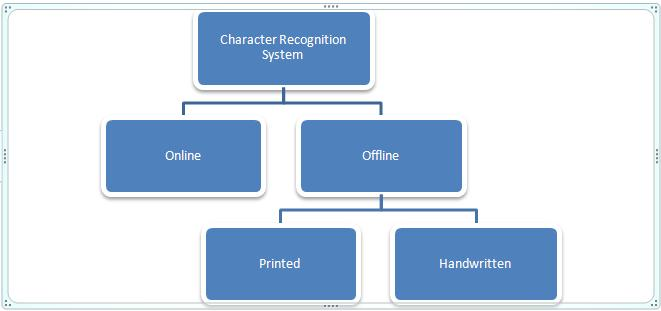
\includegraphics[scale=0.75]{images/ocr_online_offline}
\caption{Offline és Online Karakterfelismerés}
(forrás: \url{http://www.srimca.edu.in/Srijan/Srijanjan2011/IT/IntroductionToOCR.html})
\end{figure}

Az online karakterfelismerés során lehetőségünk van zaj generálására. Az ecsetvonások mozgása során véletlenszerű zajokat adhatunk hozzá. A zajos képekkel való betanítás a rendszerünk robusztusságát éri el.

Zaj hozzáadás:
\begin{itemize}
\item Pontszerű zajok: véletlenszerű fekete pixeltartomány hozzáadása
\item Elmosódások: Gauss elmosás alkalmazása
\item Forgatás: affin, perspektív transzformáció vagy forgatás origó körül 
\item Alacsony kontraszt: pixel megfelelő értékeinek szorzása
\end{itemize}

Az OCR folyamatba bevitt képek általában a szkennerekből származnak, amik általában karaktereket, ábrákat vagy egyéb, nem szöveges elemeket is tartalmazhatnak. A karakterek gyakran különböző méretűek és betűtípusokat.

Az előfeldolgozás során a következők jöhetnek szóba \cite{zhou2017stroke}: 
\begin{itemize}
\item karakterek szétosztása a bemenetek függvényében,
\item a zaj megszüntetése,
\item normalizálni a betűméretet és pozícionálni a filtert (kernel-t),
\item stroke váz generálása (thinning).
\end{itemize}

A jellemző alapú módszerek \cite{bunke1997handbook} kivonják a karakter jellemzőit, mivel ezek a jellemzők matematikailag kiszámítottak, amire alkalmas a számítógép. Így az optikai karakterfelismerés (OCR) nem igazán az optikai alapokon nyugszik, hanem inkább a matematikai számításokhoz köthető.

Amint említettem, minden kínai karakternek egyedi geometriai alakja van, amiket a stroke-ok alakítják (a stroke és az alapvonás színonim szavak). A kínai karakterek felismerésének alapja a stroke-ok és a strukturális jellemzők. Hosszú ideig ez a módszer befolyásolta a kínai karakterfelismerés kutatási irányát.
A karakter struktúrális lebontására láthatunk egy példát \aref{fig:ocr_features}. ábrán.

\begin{figure}[h]
\centering
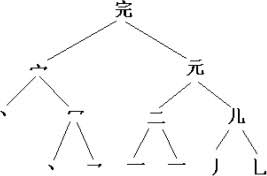
\includegraphics[scale=0.8]{images/ocr_features}
\caption{Egy kínai karakter lebontása alapelemekre, hogy az után azokat, mint jellemzőket lehessen használni}
\label{fig:ocr_features}
\end{figure}

Ennek megvalósítása nagyon nehéz a gyakorlatban, mert a stroke és a struktúrák közötti kapcsolat nagyon instabil. A stroke-ok és a strukturális jellemzők nem tudják hatékonyan kivonni a jellemzőket vagy nem praktikus.

Rengeteg mód van a jellemzők kivonására \cite{bunke1997handbook}, például lehet alapozni az él detektálásra, transzformációkra, rács jellemzőkre, kulcsfontosságú jellemzőkre, vektor vonali jellemzőkre.

Miután rendelkezésre állnak a módszerek, amikkel ki lehet nyerni a jellemzőket, hozzáfoghatunk a végleges kimenet előállítására. Lehetséges, hogy különböző felismerési rendszereket állíthat össze és összehasonlíthatjuk a kimeneteket \cite{liu2013online} \cite{dong2005improved} \cite{zhong2015high}. Azonban ez extra számítási költséget igényel, viszont a pontosság tovább javítható.

Mikor a felismerési rendszer kimenetet generál, lehetséges, hogy néhány karaktert tévesen osztályoz. Ez javítható a különböző bemeneti minták növelésével.

\subsection{Implementálás}

Egy olyan algoritmust mutatok be, ami képes kínai karakterek felismerésére sok különböző betűtípussal (pl. Song, Fang, Kai, Hei, Yuan, Lishu, Weibei és Xingkai) \cite{wu2002recognition}. Ezekre a betűtípusokra \aref{fig:chinese_fonts}. ábrán láthatunk néhány példát.

Az algoritmus származtatott jellemzőkön alapul, és egy szótár halmazt használ. Először egy 3 szintes illesztést végez mindegyik szótárhoz képest. Az ilyen illesztésekhez kapcsolódó távolsági méréseket ezután egy központi diszkriminátorba táplálják, hogy a végső felismerési eredményt kiadják. Gyors és a pontos felismerést ért el mind a címben az összes 8 betűtípust és mind a főoldalon, amelyhez az első 4 általánosan használt betűtípus tartozik.

\begin{figure}[h]
\centering
\begin{tabular}{ c c }
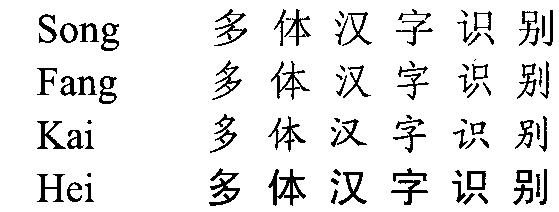
\includegraphics[scale=0.35]{images/chinese_fonts1} & 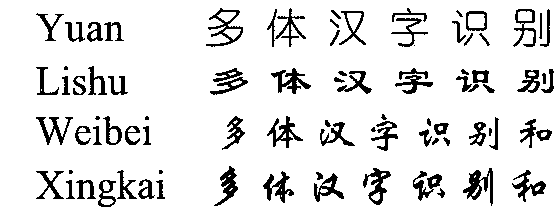
\includegraphics[scale=0.35]{images/chinese_fonts2}
\end{tabular}
\caption{Különféle kínai betűtípusok}
\label{fig:chinese_fonts}
\end{figure}

A funkciókivonás fontos eleme az OCR-nek \cite{wu2002recognition}. Az algoritmus egy 8-dimenziós vektorhoz tartozik $[d_1, d_2, \ldots d_8]$. Kiszámítása az alábbi összefüggés segítségével történik
$$
d_i = \dfrac{l_i}{\sqrt{\displaystyle \sum_{k=1}^8 l_k^2}},
$$
ahol $i = 1, \ldots, 8$, és $l_i$ a csatlakoztatott fekete képpontok száma $i$-edik irányban. Erre egy példát láthatunk \aref{fig:8direction}. ábrán.

\begin{figure}[h]
\centering
\begin{tabular}{ c c }
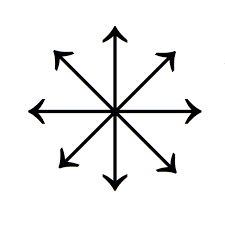
\includegraphics[scale=0.6]{images/8direction} & 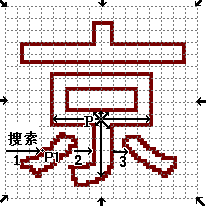
\includegraphics[scale=0.6]{images/ocr_PDC}
\end{tabular}
\caption{A jellemző irányok használati módja a karakterfelismerés során (forrás: \cite{wu2002recognition})}
\label{fig:8direction}
\end{figure}

Az OCR rendszereknél, a felismerési algoritmusok két szakaszból állnak: tanítás és tesztelés. A hálózat súlyait a képzés során határozzák meg. A képzés után a rendszer átkapcsol a tesztelési fázisra, és a szótárak szerint meghatározza a legvalószínűbb karakterindexet.

A hierarchikus illeszkedés három szintből áll. Az első szint egy osztályozó, ami felhasználja a transzformált jellemzőket. Ezután a jellemzőket egy második szintű osztályozónak adják át. Az osztályozó több elemet is kiemel (kisebb számú kimenet). A harmadik szint az összes elemet használni fogja, a karaktert a végső felismerés eredményeként kiválasztja.

A 3 szintű hierarchikus struktúra nem csak csökkenti a számítási komplexitást, hanem figyelembe veszi a jellemzők összetevőit. Az utóbbi növeli felismerési pontosságot. A 3-szintű struktúra hatékonysága a felismerési arány, a sebesség és a memória használat.

Minden tesztet két kínai mintán végzik, összesen 7510 karakterrel. Ezek az eredmények azt mutatják, hogy a 8 betűtípus átlagos felismerési aránya 99,32\% a képzési minták esetében, pedig 98,96\%. A betűtípusonként eredményeket \aref{tab:ccr_results}. táblázat foglalja össze.

\begin{table}
\centering
\begin{tabular}{ |c|c|c|c|c|c|c|c|c|c|}
\hline
Font & Song & Fang & Kai & Hei & Yuan & Lishu & Weibei & Xingkai & Average\\
\hline
Train & 99.82 & 99.64 & 99.81 & 99.57 & 98.77 & 98.75 & 99.35 & 98.82 & 99.32\\
\hline
Test & 99.71 & 99.50 & 99.80 & 99.09 & 98.43 & 98.15 & 98.78 & 98.19 & 98.96\\
\hline
\end{tabular}
\caption{Az elérhető karakterfelismerő rendszer hatékonysága különböző betűtípusok esetén (forrás: \cite{wu2002recognition})}
\label{tab:ccr_results}
\end{table}

A kísérleti eredmények azt mutatják, hogy a javasolt algoritmus képes gyorsan és pontosan felismerni a karaktereket akár 8 különböző betűtípussal is. Az algoritmus kiváló felismerési teljesítményt nyújt a 4 leggyakrabban használt betűtípusnál \cite{wu2002recognition}.

\Chapter{Jellemzők kinyerése}

% TODO: Összeszedni a jellemzően használt feature-öket. (Az előző fejezetből át lehet emelni az ide vonatkozó részeket.)

% TODO: Meg kellene nézni, hogy ebből mit és hogy lehetne implementálni \cite{trier1996feature} : http://citeseerx.ist.psu.edu/viewdoc/download?doi=10.1.1.51.7439&rep=rep1&type=pdf

% TODO: Átnézni, és kivenni a megfelelő részeket \cite{liu2008handwritten}: https://hal.inria.fr/file/index/docid/120408/filename/liama2.pdf

% TODO: \cite{liu2006high} https://hal.inria.fr/file/index/docid/120419/filename/liama4.pdf

A gépi tanulásban, a minta felismerésében és a képfeldolgozásban a funkciókivonás a mért adatok kezdeti sorozatából indul ki és nem redundáns szándékú származtatott értékeket (jellemzőket) hoz létre. A jellemzők elősegítik a későbbi tanulási és általánosítási lépéseket és egyes esetekben a jobb emberi értelmezést. A funkciókivonás\cite{features27:online} összefügg a dimenzionalitás csökkentésével.

Ha egy algoritmushoz tartozó bemeneti adat túl nagy ahhoz, hogy feldolgozni lehessen, mert gyaníthatóan redundáns (pl. a képpontként ismétlődése a megjelenített képeken), akkor átalakítható egy csökkentett készletté (funkcióvektorként is nevezik). A kezdeti funkciók egy részhalmazának meghatározása a funkciókiválasztásnak nevezik. A kiválasztott funkciók várhatóan tartalmazzák a bemeneti adatok releváns adatait, így a kívánt feladat a teljes kezdeti adat helyett a csökkentett ábrázolás használatával végezhető el.

\section{Dimenzió redukció}
\begin{itemize}
\item PCA: A dimenziócsökkentés\cite{wang2003feature} fő lineáris technikája a főkomponens elemzés, az adatok lineáris leképezését végzi egy alsó dimenziós térben. A főkomponens-elemzés (PCA) az osztályozási problémák dimenzió csökkentési technikájaként használható. A dimenziócsökkentés fő lineáris technikája, főkomponens elemzés, az adatok lineáris leképezését végzi egy alsó dimenziós térben.

A gyakorlatban az adatok kovariancia mátrixát állítják össze és a mátrixban lévő sajátvektorokat kiszámítják. A legnagyobb sajátértékeknek megfelelő sajátvektorok a főkomponensek, amelyek felhasználhatók az eredeti adatok nagy részének rekonstruálására.

Ha létezik egy $A$ nevű négyzetes mátrix, egy skalár $\lambda$ és egy nem nulla vektor $v$, akkor $\lambda$ az sajátérték és a $v$ a sajátvektor, ha a következő egyenlet teljesül:

$$
Av = \lambda v
$$

\item Kernel PCA: A fő komponenselemzés nemlineáris módon használható az úgynevezett kernel trükkel. Az így kapott technika képes nemlineáris leképezések létrehozására, amelyek maximalizálják az adatokban a varianciát.

Példa egy lineárisan nem szeparálható adathalmazra \aref{fig:kernel_pca_input} ábrán látható:

\begin{figure}[h]
\centering
\captionsetup{justification=centering}
\begin{tabular}{ c c }
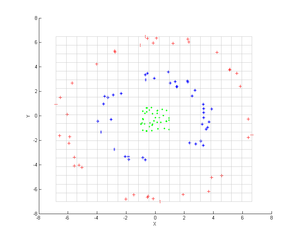
\includegraphics[scale=0.8]{images/kernel_pca_input} & 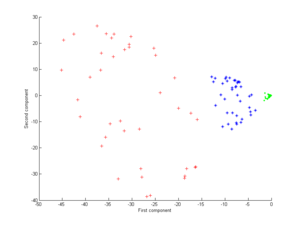
\includegraphics[scale=0.8]{images/kernel_pca_output}
\end{tabular}
\caption[caption]{Bementi pontok kernel PCA transzformáció után
\hspace{\textwidth}Forrás:\url{https://en.wikipedia.org/wiki/Kernel_principal_component_analysis}}
\label{fig:kernel_pca_input}
\end{figure}

\Aref{fig:kernel_pca_input} ábra bal oldali képen az adatok lineárisan nem szeparálhatók. A kernel PCA transzformáció során olyan teret képezünk le (\aref{fig:kernel_pca_input} ábra jobb oldali kép), ahol az adatok lineáris leképezés lehetséges.

A kernel meghatározása:
$$
k({\boldsymbol  {x}},{\boldsymbol  {y}})=({\boldsymbol  {x}}^{{\mathrm  {T}}}{\boldsymbol  {y}}+1)^{2}
$$

Lehetőségünk van különböző kernelek definiálására, felsorolok néhány példát: \textit{Gauss kernel:} $e^{{\frac  {-||{\boldsymbol  {x}}-{\boldsymbol  {y}}||^{2}}{2\sigma ^{2}}}}$ \textit{, Tangens kernel:} $tanh(({\bf x}\cdot {\bf y})+\theta)$ \textit{, Polinom kernel:} $({\bf x}\cdot {\bf y})^k$

\item LDA\cite{wang2003feature}: A lineáris diszkriminancia-analízis (LDA) a Fisher lineáris diszkriminánsának, a statisztikában, a minta felismerésében és a gépi tanulásban használt módszer, amely olyan objektumok lineáris kombinációját találja, amely két vagy több objektum- vagy eseményosztályt jellemez vagy elválaszt.
\item Autoencoder: Az "autoencoding" egy olyan adattömörítési algoritmus, ahol a tömörítési és dekompressziós függvények:
\begin{enumerate}
\item adat-specifikusak: Az autoencoderek adatspecifikusak, ami azt jelenti, hogy csak azokat az adatokat tudják tömöríteni, amelyekkel betanították.
\item veszteségesek: Az autoencoderek veszteségesek, ami azt jelenti, hogy a dekompresszált kimenetek az eredeti bemenetekhez képest romlanak.
\item automatikusan tanul: Tanulnak a példákból, nem pedig ember által előtervezettek.
\end{enumerate}
Minden olyan környezetben, ahol az "autoencodert" használják, a kompressziós és dekompressziós funkciókat neurális hálózatokkal valósítják meg.

Ma az autoencoderek két érdekes gyakorlati alkalmazása az adatok zajszűrése és az adatok dimenziócsökkentése. Megfelelő dimenzionalitással az autoencoderek jobban teljesítenek mint a PCA vagy egyéb alapvető technikák.

Az autoencoder implementálása a \textit{keras} könyvtár, a  \textit{layers} és \textit{models} modulok használatával:
\begin{python}

input_img = Input(shape=(784,)) # A bemeneti adat
encoded = Dense(32, activation='relu')(input_img) # kodolt adat
decoded = Dense(784, activation='sigmoid')(encoded) # dekodolt adat
# Az autoencoder, encoder, decoder modell
autoencoder = Model(input_img, decoded)
encoder = Model(input_img, encoded)
encoded_input = Input(shape=(32,))
decoder_layer = autoencoder.layers[-1] # Autoencoder utolsó rétege
decoder = Model(encoded_input, decoder_layer(encoded_input))
\end{python}
\begin{python}
autoencoder.compile(optimizer='adadelta', loss='binary_crossentropy')
\end{python}
A fordítás után következhet a tanítás
\begin{python}
autoencoder.fit(x_train, x_train,	# A tanito es a cel
                epochs=50,		# adatok megegyeznek
                batch_size=256,
                shuffle=True,
                validation_data=(x_test, x_test))
\end{python}
\end{itemize}

A neurális hálózat szerkezete \aref{fig:deep_autoencoder} ábrán látható:
\begin{figure}[h]
\centering
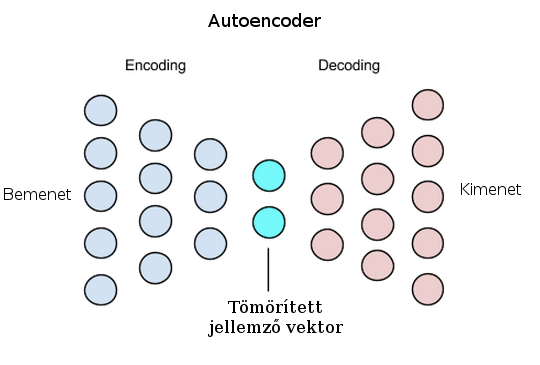
\includegraphics[scale=0.6]{images/deep_autoencoder}
\caption{Autoencoder}
\label{fig:deep_autoencoder}
\end{figure}

A neurális hálózatunk szimmetrikus. A középső rejtett rétegen az adatunk tömörített változatát találhatjuk. Számunkra nem a kimenet az érdekes, hiszen az csak egy másolata a bementi rétegnek. A rejtett rétegek súlyai fontosak számunkra. Az előállított súlyokkal képesek vagyunk az adatok dimenzió csökkentésére. A kép egy tömörített változata elősegíti a gyorsabb feldolgozást.

\section{Alacsony szintű jellemzők}
Az alacsony szintű jellemző\cite{features27:online}, amelyek a kép tartalmát leíró technikák, egy teljes kép szintjén, nem pedig annak különböző területein. Az egyik legfontosabb folyamat, amellyel találkozunk, az úgynevezett éldetektálás.
\begin{itemize}
\item Éldetektálás: Az éldetektálás számos matematikai módszert foglal magában, amelyek olyan pontok azonosítását célozzák meg egy digitális képen, amelyeknél a kép fényereje élesen megváltozik vagy formálisan megszakad. Azok a pontok, amelyeknél a kép fényereje élesen változik, tipikusan íves szegmensek csoportjába sorolják.
Kép fényerejének hirtelen változásainak okai lehetnek:
\begin{enumerate}
\item Hirtelen mélységi változás
\item Felület normálisának változása
\item Megvilágítás változása: árnyékok, világítás változás
\item Visszaverődésben változás: felület tulajdonság
\end{enumerate}
\item Sarokérzékelés: A sarokérzékelés egy olyan megközelítés, amelyet a számítógépeslátásnál használnak bizonyos jellemzők kivonására és a kép tartalmának kivonására.
A sarok két él metszéspontjaként definiálható. A sarok olyan pontként is definiálható, amelynél a pont egy helyi szomszédságában két domináns és különböző él irány található.
Harris és Stephens sarokdetektáló algoritmus rendkivül gyors. A szürkeárnyalatos kétdimenziós képeknél alkalmazhatjuk. Adjuk meg ezt a képet $I$ segítségével. Vegyünk egy képpontot a $(u, v)$ területen és mozgassuk azt $(x, y)$. A két pont közötti négyzetes különbség (SSD) súlyozott összege, $S$, az alábbiak szerint adható meg:

$$
S(x,y)=\sum_{u}\sum_{v}w(u,v)(I(u+x,v+y)-I(u,v))^{2}
$$

A Harris mátrix:

$$
{\displaystyle A=\sum _{u}\sum _{v}w(u,v){\begin{bmatrix}I_{x}(u,v)^{2}&I_{x}(u,v)I_{y}(u,v)\\I_{x}(u,v)I_{y}(u,v)&I_{y}(u,v)^{2}\end{bmatrix}}={\begin{bmatrix}\langle I_{x}^{2}\rangle &\langle I_{x}I_{y}\rangle \\\langle I_{x}I_{y}\rangle &\langle I_{y}^{2}\rangle \end{bmatrix}}}
$$

Ahol:\\
$I_x$: Az adott derivált az x-irányban\\
$I_y$: Az adott derivált az y-irányban\\
$w(x, y)$: Súlyozási függvény (pl. Gaussian)

Egy sarkot az $(x, y)$ vektor minden irányának $S$ változata jellemez. Az $A$ sajátértékének elemzésével ezt a jellemzést a következő módon fejezhetjük ki: $A$-nak két sajátértékkel kell rendelkeznie egy sarok pontra. A sajátértékek nagyságrendje alapján az alábbi következtetésekre lehet következtetni:
\begin{enumerate}
\item Ha $\lambda _{1}\approx 0$ és $\lambda_2 \approx 0$ akkor az $(x,y)$ képpontnak nincs sarok jellemzője.
\item Ha $\lambda_1 \approx 0$ és $\lambda _{2}$ egy nagy pozítiv szám, akkor sarok található.
\item Ha $\lambda_1$ és $\lambda_2$ nagy pozítiv szám, akkor sarok detektálható.
\end{enumerate}
\item Méret-invariáns jellemző transzformáció (SIFT): A transzformáció a számítógéplátásban használt algoritmus, amely helyi jellemzők felderítésére és leírására használják. A kulcspontokat az objektumokon először egy kép készletből vonják ki és tárolják egy adatbázisban. Egy objektumot felismerünk egy új képen azáltal, hogy az egyes képeket az új képből az adatbázisba hasonlítjuk össze és megtaláljuk a megfelelő jellemzőket, amelyek euklideszi távolságukon alapulnak. \Aref{fig:sift} ábrán látható egy példa.
\begin{figure}[h]
\centering
\captionsetup{justification=centering}
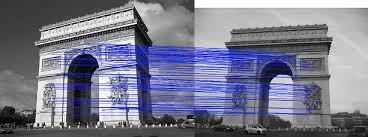
\includegraphics[scale=1.0]{images/sift}
\caption{A jellemzők felderítése elforgatott képen \hspace{\textwidth}Forrás:\url{http://www.ismailsirma.com/visualsfm-3d-construction-of-images}}
\label{fig:sift}
\end{figure}
\end{itemize}

\section{Irány szerinti jellemző kinyerés}
Figyelembe véve, hogy a kínai karakterek stroke részei megközelíthetők többféle irányba. A korai munkákban négy irányba (vertikális, horizontális, bal átlós és jobb átlós) bontották fel a karaktereket. A képpontok nyolc irányba történő bontása (\aref{fig:direction8} ábra) négy irány helyett jelentősen javította a felismerési pontosságot. Ez azért van így, mert a stroke két oldalának elválasztása jobban megkülönbözteti a párhuzamos stroke-okat.

\begin{figure}[h]
\centering
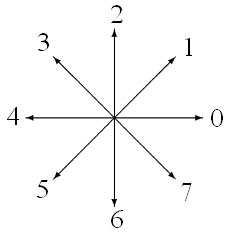
\includegraphics[scale=0.5]{images/direction8}
\caption{8 irányú felbontás}
\label{fig:direction8}
\end{figure}

Az irány funkciók kinyerése\cite{liu2008handwritten} három lépésben valósul meg: kép normalizálása, irány dekompozíció és jellemző mintavételezés. 

A normalizálás szabályozza a karakterek kép méretét, pozícióját és alakját, hogy csökkentse az azonos osztályú képek közötti változatokat.

\subsection{Irány dekompozíció}

Az irány dekompozíció több iránysíkot eredményez, $f_i(x, y), i = 1,. . . , N_d$. Először leírjuk a gradiens dekompozícióra szolgáló eljárásokat 8 irányban, majd kiterjeszük 12 és 16 irányba.

A gradiens irányú jellemző kinyerés a gradiensvektor, amelyet a normalizált képen számolunk ki a Sobel operátorral, ami 8 irányra bontja a komponenseket. A Sobel operátornak két maszkja van, hogy kiszámítsa a gradiens komponensek a két tengelyen. A maszkok \aref{fig:sobel_operator} ábrán látható.

\begin{figure}[h]
\centering
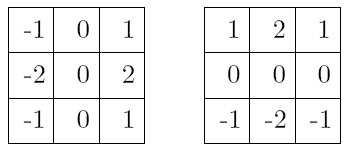
\includegraphics[scale=0.5]{images/sobel_operator}
\caption{Sobel operátor}
\label{fig:sobel_operator}
\end{figure}

Ha egy gradiens irány két standard irány között fekszik, akkor a vektor két komponensre bomlik. Az egyes komponensek hossza a (x, y) képponthoz tartozó megfelelő irány síkhoz van hozzárendelve.

\subsection{Elmosódás és mintavétel}

Mindegyik irány síkot, amelynek méretével megegyezik a normalizált kép azt csökkenteni kell, hogy mérsékelt dimenziójú jellemző értékeket nyerjen. Egy egyszerű módja az, hogy az irány síkot több blokkzónába osztjuk és az egyes zónák teljes vagy átlagos értékét jellemző értékként vesszük.

Az elmosódás végrehajtásakor a térbeli szűrő impulzus-válaszfüggvénye (IRF) egy súlyozott ablakhoz hasonlít, amelyet elmosódási maszknak is neveznek. Az IRF-t gyakran Gaussian függvényként veszik figyelembe:

$$
g(x,y) = \frac{1}{\sqrt{2\pi}\sigma} e^{{(- \frac{x^2 + y^2}{2 \sigma_x^2})}}
$$

A mintavételi tétel szerint a $\sigma_x$ variancia-paraméter a mintavételi frekvenciához kapcsolódik. A Gauss-szűrő sávszélességének az empirikus képlet az alábbi $\sigma_x = \frac{\sqrt{2}t_x}{\pi}$, ahol $t_x$ a mintavételi intervallum.

A kivont jellemzőértékek változók. A transzformáció az változók sűrűségfüggvényét közelebb hozhatja a Gaussian függvényhez. Ez segít a statisztikai osztályozás teljesítményének javításában.

\subsection{Számítási idők}
A jellemző kinyerés CPU időtartama szinte független a normalizációs módszertől. Két részből áll: irány dekompozíció és elmosódás. A három irányú jellemzők átlagos CPU-ideje
\aref{cpu_times} táblázat mutatja. Az elmosódás feldolgozási ideje függ az irányok szűkösségétől (a nulla pixeleket nem veszi figyelembe).

\begin{table}[h]
\centering
\caption{CPU idők}
\label{cpu_times}
\begin{tabular}{|l|l|r|}
\hline
\multicolumn{1}{|c|}{} & direction & blurring \\ \hline
chn                    & 0.121     & 0.439    \\ \hline
nccf                   & 0.458     & 0.752    \\ \hline
grd-g                  & 0.329     & 1.276    \\ \hline
\end{tabular}
\end{table}

\subsection{Korlátozás nélküli minták}
A korlátozás nélküli kézzel készített mintákkal rendelkező képzési osztályozók képesek lesznek javítani a korlátozás nélküli karakterfelismerés pontosságát. A korlátozás nélküli karakterek nagy adatbázisának gyűjtése sürgős feladat lesz a közeljövőben.

Ha a hibaarányt meglehetősen alacsony szintre szeretné csökkenteni (például 2\% -ot az elszigetelt karakterek esetében), egyszerűen csak az aktuális normalizációs és funkciókivonási módszerek használata nem elegendőek. A normalizálás, a funkciókivonás és az osztályozó kialakításának módszereit újra kell gondolni a írásjelek jobb felismerésére. A képzési osztályozók diszkriminatív módon javíthatják a kézírásos és a korlátozás nélküli karakterfelismerés pontosságát.
\Chapter{Konvolúciós neurális hálók}

% TODO: Az általános ANN-t épp csak említés, áttekintés szintjén kellene bemutatni.

% TODO: Konvolúciós hálók alkalmazásához kapcsolódóan feldolgozni pár cikket.

% TODO: Átnézni, hogy van-e benne jó hivatkozás: http://papers.nips.cc/paper/6637-gated-recurrent-convolution-neural-network-for-ocr.pdf

% TODO: Lehetséges topológiákra tenni javaslatokat.

\section{Neurális hálók}

A neurális hálózattokat \cite{neuralis77} gyakran hasonlítjuk az emberi agy működéséhez. Ha körültekintően szemügyre vesszük agyunk működését, akkor azt tapasztaljuk, hogy neuronokból és közöttük felépülő kapcsolatokból áll össze. A külvilágból érkezett ingereket értelmezhetjük úgy, mint egy bemenetet, amit az agyunkban lévő neuronok feldolgoznak.

A neurális hálózatot alkotó neuronok úgynevezett rétegekbe rendeződnek. Háromféle réteget különbözetünk meg, a \textbf{\textit{bemeneti}}, a \textbf{\textit{kimeneti}} és a \textbf{\textit{rejtett réteget}}. Bemeneti és kimeneti rétegből minden hálózatban egy darab van, rejtett rétegből azonban tetszőleges számú lehet.

A hálózatban a rétegeket élek kötik össze egymással, amelyekhez egyenként egy-egy \textbf{\textit{súly}} tartozik. A neuronok a bemeneti éleiken kapott értékek és a súlyok segítségével bizonyos műveleteket végeznek el, majd az eredmény a kimeneti éleiken keresztül továbbítják a következő réteg neuronjai felé.

\subsection{A neurális hálók elemei}

Az egyszerűség kedvéért vizsgáljunk meg egy olyan neurális hálózatot, amelynek egyetlen neuronnal rendelkezik. Ezt szokás \textbf{\textit{Perceptron}}-nak is nevezni.

\textbf{\textit{Bemenet}}: Az kiértékelendő adat (ember számára ingerek), amit általában egy vektor (jelölje $x$) reprezentál.

\textit{\textbf{Súlyok}}: Két neuron közötti kapcsolat. Egy valós érték. A hálózat súlyait mátrixba tároljuk el (ezt jelölje $W$).

\textbf{\textit{Összegző csomópont}}: A bemeneteket összeszorozza a megfelelő súlyokkal és ezek összegét képezi. Tulajdonképpen mátrix szorzásról van szó.

$$
v(n) = \sum_{i=1}^{n}(w_ix_i)
$$

\textit{\textbf{Aktivációs függvény}}: Egy olyan függvény ($\varphi$), ami leképezi a kapott összeget egy adott intervallumba, amely általában a $[0, 1]$ vagy $[-1, 1]$ intervallumokat jelenti.

\textbf{\textit{Kimenet}}: A leképezett értékünk lesz a kimenetünk (jelölje $y$).

\begin{figure}[h]
	\centering
	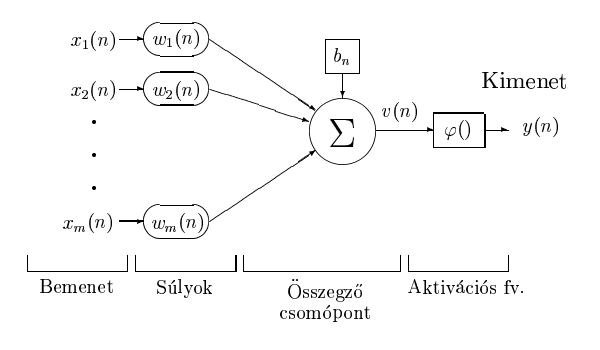
\includegraphics[scale=0.6]{images/ANNParts.png}
	\caption{A matematikai neuron modell felépítése (forrás: \cite{neuralis77})}
	\label{fig:ANNParts}
\end{figure}

\Aref{fig:ANNParts}. ábrán láthatjuk a mesterséges neurális háló neuronjának matematikai modelljét.

Amennyiben az $x(n)$ bemenethez tartozó ideális kimenetet $d(n)$-nel jelöljük, illetve $y(n)$ jelenti a hálózat által az $x(n)$ bemenetre adott kimenetét, a neurális hálózat négyzetes hibáját a következőképpen értelmezzük:
$$
\varepsilon = (d(n) - y(n))^2.
$$

Ezt a hibát akarjuk a tanítási eljárás során minimálisra csökkenteni. Természetesen az lenne az ideális, ha a hibát egészen nullára tudnánk redukálni, de ez általában nem sikerül, ezért meg kell elégednünk egy kellően kicsiny hibaküszöbbel.

Aktivációs függvénynek általában a szigmoid, azaz S alakú, függvényeket használjuk (mint például a logisztikus, tangens hiperbolikus függvények).

Az aktivációs függvényeknél egy úgynevezett rámpafüggvényről (RELU), ami az
$$
f(x) = max(0,x)
$$
összefüggéssel írható le, ahol $x$ az aktivációs függvény bemenete (\ref{fig:relu}. ábra).

\begin{figure}[h]
\centering
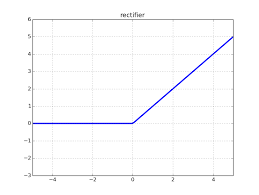
\includegraphics[scale=1.0]{images/relu}
\caption{A rámpafüggvény}
\label{fig:relu}
(forrás: \url{https://sefiks.com/2017/08/21/relu-as-neural-networks-activation-function/})
\end{figure}

A legújabb biológiai kutatások és a gyakorlati tapasztalatok is igazolják hogy a RELU-val történő tanítások szignifikánsan jobban teljesítenek. Legnagyobb előnye a regressziós tanítások esetén mutatkozik meg.

\section{A Backpropagation tanítási algoritmus}

Hiba minimalizálása során szükségünk van az aktuális hibára. Az összes kimeneti neuronra kiszámoljuk a négyzetes hibát Wés ezeket összeadjuk:
$$
E_{total} = \sum \dfrac{1}{2}(target - output)^2.
$$
(Az $\dfrac{1}{2}$ szorzót azért használjuk hogy el tudjuk távolítani majd a kitevőt a későbbiekben deriváláskor.)

A backpropagation célja, hogy frissítse az egyes súlyokat a hálózaton úgy, hogy az aktuális kimenet közelebb kerüljön a célkimenethez, ezáltal minimalizálva az egyes kimeneti neuronok és a hálózat egészének hibáját. A backpropagation algoritmus számításaira láthatunk egy példát \aref{fig:ANN_backprog}. ábrán.

\begin{figure}[h]
\centering
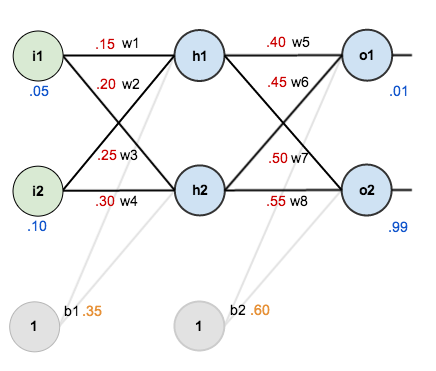
\includegraphics[scale=0.5]{images/ANN_backprog}
\caption{Példa a visszaterjesztéses tanítás alkalmazására}
(forrás: \url{https://mattmazur.com/2015/03/17/a-step-by-step-backpropagation-example/})
\label{fig:ANN_backprog}
\end{figure}

Tekintsük a $w_5$-öt. Azt szeretnénk tudni, hogy a $w_5$ változása milyen hatást gyakorol a teljes hibára, más néven $\frac{\partial E_ {total}}{\partial w_ {5}}$. Úgy is fogalmazhatunk hogy a gradiens a $w_5$ vonatkoztatásba.

Ezt a láncszabály alkalmazásával tudjuk kiszámolni:
$$
\frac{\partial E_{total}}{\partial w_{5}} = \frac{\partial E_{total}}{\partial out_{o1}} \cdot \frac{\partial out_{o1}}{\partial net_{o1}} \cdot \frac{\partial net_{o1}}{\partial w_{5}}.
$$

Lássuk az egyenlet elemeit!
\begin{flushleft}
\begin{equation}
E_{total} = \frac{1}{2}(target_{o1} - out_{o1})^{2} + \frac{1}{2}(target_{o2} - out_{o2})^{2}
\end{equation}
\begin{equation}
\frac{\partial E_{total}}{\partial out_{o1}} = 2 \cdot \frac{1}{2}(target_{o1} - out_{o1})^{2 - 1} \cdot (-1) + 0
\end{equation}
\begin{equation}
\frac{\partial E_{total}}{\partial out_{o1}} = -(target_{o1} - out_{o1}) = -(0.01 - 0.75136507) = 0.74136507
\end{equation}

\end{flushleft}

A logisztikus függvény parciális deriváltja a kimenet szorzata (1 - kimenet):
$$
out_{o1} = \frac{1}{1+e^{-net_{o1}}}
$$

$$
\frac{\partial out_{o1}}{\partial net_{o1}} = out_{o1}(1 - out_{o1}) = 0.75136507(1 - 0.75136507) = 0.186815602
$$

Végül, mennyire változik az $o1$ változó teljes bemenete a $w_5$ tekintetében?
$$
net_{o1} = w_5 \cdot out_{h1} + w_6 \cdot out_{h2} + b_2 \cdot 1
$$

$$
\frac{\partial net_{o1}}{\partial w_{5}} = 1 \cdot out_{h1} \cdot w_5^{(1 - 1)} + 0 + 0 = out_{h1} = 0.593269992
$$

Összesítve az eddigieket:
$$
\frac{\partial E_{total}}{\partial w_{5}} = \frac{\partial E_{total}}{\partial out_{o1}} \cdot \frac{\partial out_{o1}}{\partial net_{o1}} \cdot \frac{\partial net_{o1}}{\partial w_{5}}
$$

$$
\frac{\partial E_{total}}{\partial w_{5}} = 0.74136507 \cdot 0.186815602 \cdot 0.593269992 = 0.082167041
$$

A hiba csökkentése érdekében kivonjuk ezt az értéket az aktuális súlyból (adott esetben szorozva egy bizonyos tanulási sebességgel, $\eta$, amelyet 0,5-re állítunk):
$$
w_5^{+} = w_5 - \eta \cdot \frac{\partial E_{total}}{\partial w_{5}} = 0.4 - 0.5 \cdot 0.082167041 = 0.35891648
$$

Meg tudjuk ismételni ezt a folyamatot, hogy megkapjuk az új súlyokat $w_6$, $w_7$ és $w_8$:
$$
w_6 ^ {+} = 0,408666186
$$

$$
w_7 ^ {+} = 0.511301270
$$

$$
w_8 ^ {+} = 0.561370121
$$

Ezután folytatjuk a hátrafelé az új értékeket a $w_1$, $w_2$, $w_3$ és $w_4$ értékek kiszámításával. Hasonlóan láncszabályt alkalmazunk. A visszaterjesztés módjának egy szemléltetését \aref{fig:ANN_bp_viz}. ábrán láthatjuk.

\begin{figure}[h]
\centering
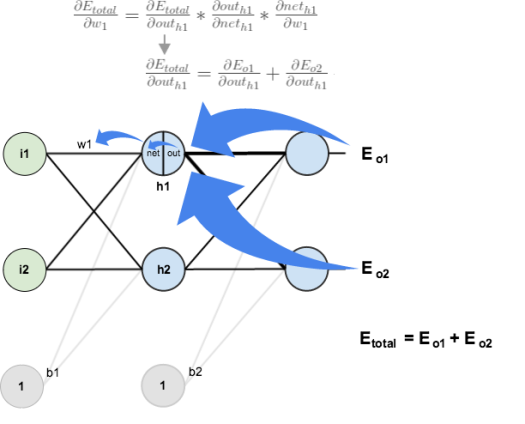
\includegraphics[scale=0.5]{images/ANN_bp_viz}
\caption{A hiba visszaterjesztése a súlyok módosításához}
\label{fig:ANN_bp_viz}
(forrás: \url{https://mattmazur.com/2015/03/17/a-step-by-step-backpropagation-example/})
\end{figure}

Végül frissítjük az összes súlyunkat. Amikor eredetileg a 0.05 és a 0.1 bemeneteket továbbítottuk, a hálózat hibája 0.2983711 volt. A backpropagation első fordulója után a teljes hiba 0.2910279 értékre csökken. Lehet, hogy nem tűnik soknak, de miután megismételtük ezt a folyamatot 10 000-szer, a hiba lecsökken 0.0000351-re.

\section{Konvolúciós neurális hálózat}

A konvolúciós neurális hálózat hagyományos neurális hálózat alapokon nyugszik \cite{liconvolution}. Annak egy speciális fajtája, amit képeken található minták feltárására fejlesztettek. Neuronokból épülnek fel és hasonlóképpen rendelkeznek tanítható súlyokkal. A bemeneteiken kapott értékek skaláris szorzatát egy nem lineáris leképezés követheti. Az egész hálózat reprezentálhat egy egyszerű osztályozó eljárást, aminek a bemenetei a nyers képpontok és a kimenete lehet egy adott kép osztályba tartozás valószínűsége. A mi esetünkbe a bemenet a kínai karakter pixel értékei, a kimenet pedig valószíűségek a karakterekből adódóan.

A konvolúciós neurális hálózat hagyományos neurális hálózat alapokon nyugszik. Annak egy speciális fajtája, amit eredendően képeken található minták feltárására fejlesztettek. Neuronokból épülnek fel és hasonlóképpen rendelkeznek tanítható súlyokkal. A bemeneteiken kapott értékek skaláris szorzatát egy nem lineáris leképezés követheti. Az egész hálózat reprezentálhat egy egyszerű osztályozó eljárást, aminek a bemenetei a nyers képpontok és a kimenete lehet egy adott kép osztályba tartozás valószínűsége. A mi esetünkben a bemenet a kínai karakterek pixel értékei, a kimenet pedig egy becsült osztályba tartozási mérték.

A hagyományos neurális hálózatok nem skálázzák a teljes képet. A kínai (különösen a hagyományos) több száz karaktert nem lehet megjeleníteni egy $16 \times 16$ pixeles rácsban. A megfelelő méret körülbelül $24 \times 24$ képpontot tartalmaz. Neurononként $24 \times 24 = 526$ súly paramétert jelentene. Ez még kezelhetőnek tűnik, de tisztán látszik, hogy a teljesen összekapcsolt struktúra nem kezeli jól a képeket.

Ha végig gondoljuk, hogy az hány paramétert jelent még egy kis neuronszámú kevés rejtett rétegből álló hálózat esetében, akkor rájöhetünk, hogy nagyobb méretű képen fellelhető minták felismeréséhez a hagyományos neurális hálózatok alkalmazása nem célravezető, emiatt a kép előfeldolgozására, szűrésére konvolúciós rétegeket vezetnek be.

\subsection{A háló felépítése}

A konvolúciós neurális hálózatokban szereplő rétegeket funkció alapján alapvetően két csoportra lehet bontani.

\begin{enumerate}
\item A konvolúciós rétegek, amik - mint paraméterezhető szűrők - előfeldolgozást végeznek a képen. Ezáltal a kép mérete lecsökken, a hordozott információtartalom kiemeltté válik.
\item A hagyományos neurális hálózat (második csoport) számára feldolgozható lesz, az osztályozást el tudja végezni. Egy konvolúciós neurális hálózat tehát konvolúciós és hagyományos rejtett rétegekből épül fel.
\end{enumerate}

A konvolúciós rétegek alapjában véve színes képek feldolgozására lettek kifejlesztve, ezért a neuronjaik három dimenzióban (szélesség, magasság, színcsatornák) vannak elrendezve.

A mi esetünkbe fekete-fehér képek állnak rendelkezésre. A színes képek esetén grayscale konvertálást végezhetünk el. Ha a pixel érték fekete akkor 0-át, ha fehér akkor 255-et rendelünk hozzá. A szürke árnyalatokat $[0, 255]$ közötti értékekkel definiáljuk. Egy kínai karakterre \aref{fig:chinese_char_pixel}. ábrán láthatunk példát.

\begin{figure}[h]
\centering
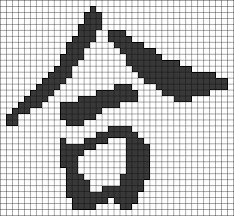
\includegraphics[scale=0.65]{images/chinese_char_pixel}
\caption{Egy kínai karakter fekete-fehér raszteres képként}
\label{fig:chinese_char_pixel}
\end{figure}

A következő felsorolásban - a tipikus, de nem kizárólagos sorrendre ügyelve - bemutatnám a konvolúciós hálózat rétegtípusait:

\begin{itemize}
\item \textit{Bemeneti réteg}: Tartalmazza a kép nyers pixel értékeit. Az értékeket sorba állítjuk és azokat egy 1 dimenziós vektor reprezentálja, ami 0 és 1 értékeket tartalmaz.

\item \textit{Konvolúciós réteg}: Adott képpont csoportokra konvolúció matematikai műveletet alkalmazunk. A konvolúció eredménye egy skalár (a skaláris szorzata a kép egy adott részének és a szűrőnek). Ha minden képpont csoportra elvégezzük a konvolúciót, akkor egy aktivációs térképet kapunk. Általában több szűrő paraméterrel is elvégezzük a konvolúciót és aktivációs térképeket egymásra rakjuk. Az aktivációs térkép, a művelet tulajdonsága miatt, kisebb
méretű lesz (\ref{fig:convolution}. ábra).

\begin{figure}[h]
\centering
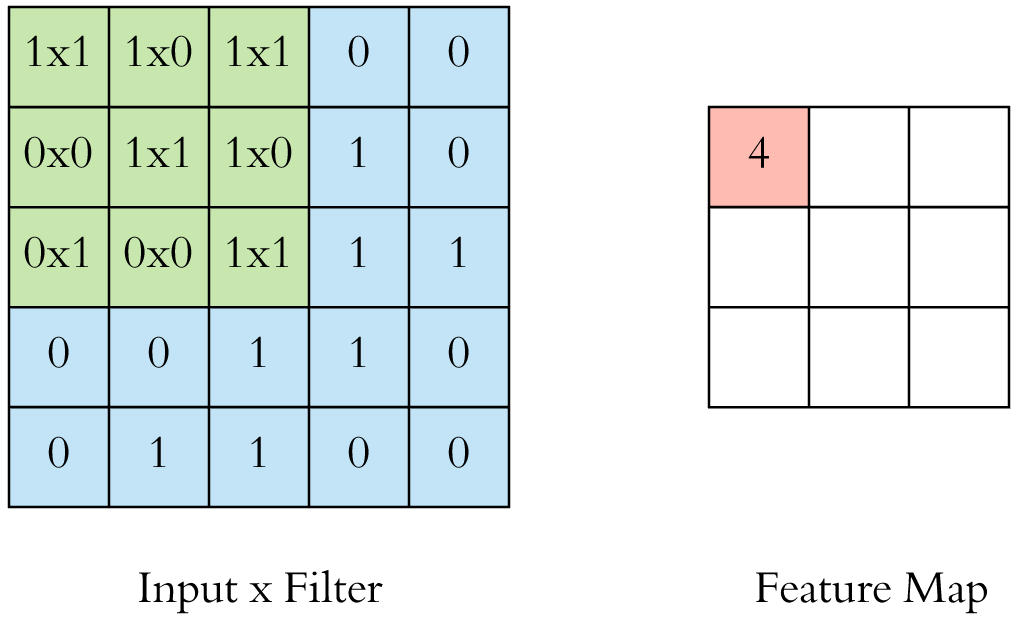
\includegraphics[scale=0.3]{images/convolution}
\caption{A bináris mátrix és a belőle konvolúcióval kinyert jellemzők}
(forrás: \url{https://towardsdatascience.com/applied-deep-learning-part-4-convolutional-neural-networks-584bc134c1e2})
\label{fig:convolution}
\end{figure}

Konkrétan mátrix szorzásról van szó. A feature map elemei egész számok, amik további konvolúciós rétegen mennek keresztül. Lehet közben különböző szűröket is használni.

\item \textit{RELU réteg}: A konvolúciós réteg aktivációs függvénye, ami a következő leképezést valósítja meg: $f(x) = max(x, 0)$. Vagyis, ha a bemenet kisebb, mint nulla, akkor a kimenet nulla lesz, ha nagyobb, mint nulla, akkor a kimenet a bemenet értékét veszi fel. A konvolúciós hálóknál a RELU sokkal gyorsabb más aktivációs függvényeknél, mint például a sigmoid vagy a tanh.
\item \textit{Összevonó réteg (pooling layer)}: A Pooling Layer függetlenül működik minden egyes feature map-nél. A MAX művelet segítségével kinyeri a legfontosabb vonásokat, csökkentve a dimenzióját. A leggyakoribb forma egy $2 \times 2$-es méretű szűrő, melyet 2 lépéssel kell felvinni minden szeletre. A bemenetben 2 szélesség és magasság mellett, az aktiválások 75\% -át eldobja. Minden MAX művelet ebben az esetben 4 számot vesz igénybe.

\begin{figure}[h]
\centering
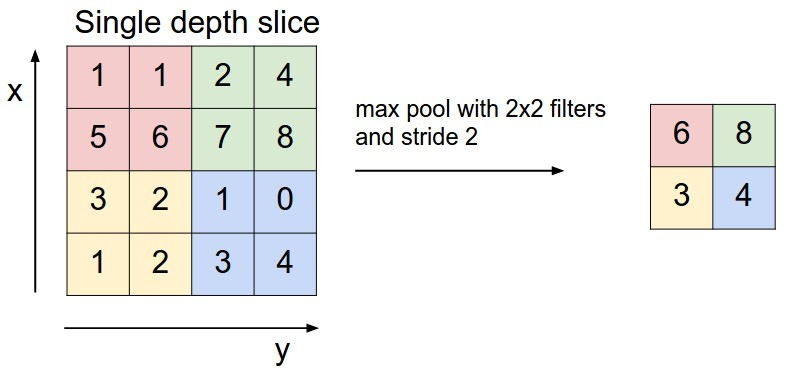
\includegraphics[scale=0.3]{images/maxpool}
\caption{A pooling réteg működése egy példán keresztül}
\label{fig:maxpool}
(forrás: \url{http://cs231n.github.io/convolutional-networks/})
\end{figure}

\item \textit{Teljesen összekötött réteg (fully connected, FC)}: Utolsó rétegekként szokták használni, hagyományos réteg. Lehet 1 vagy több réteg is a feladattól függően. Az osztályozás rész itt történik. A kimenetek valószínűségek a felsorolt karakterek szerint.
\end{itemize}

\Aref{fig:CNN_CCR_working}. ábra egy konvolúciós feldolgozást mutat be, ahol szemléltetve vannak az egyes rétegek utáni állapotok. A képen látható az egyes konvolúció utáni állapotok tulajdonság érzékelőként viselkednek.

\begin{figure}[h]
\centering
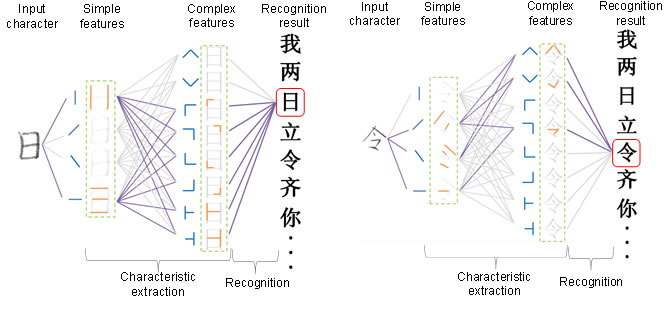
\includegraphics[scale=0.65]{images/CNN_CCR_working}
\caption{A konvolúciós karakterfelismerő hálózat sematikus felépítése}
(forrás: \url{http://www.fujitsu.com/global/Images/20130821-01b_tcm100-929717.jpg})
\label{fig:CNN_CCR_working}
\end{figure}

\subsection{Hálózat architektúra}

A megfelelő háló architektúra megválasztása nagyon fontos a tervezési szakasznál. A következőkben egy 2013-as eredményt mutatok be, miszerint a rétegek és a bennük lévő neuronok számával csökkenthető a hibaarány \cite{cirecsan2015multi}.

Először vessünk egy pillantást az adathalmazunkra. Az adat egyszerű képeket tartalmaz (offline kép). Tartalmaz 224419 karaktert, amelyeket 60 személy írt. A karakterek $48 \times 48$ pixelre skálázták. Az előfeldolgozás OpenCV-vel történik.

Nyolc hálózaton történt tanítás. Minden hálózatnak 11 rétege van, beleértve a bemeneti és kimeneti réteget. A jellemzők kinyerés fázisánál 100-450 darabszámú neuront használ. Végezetül két egymást követő teljesen összekötött (fully-connected) hálózat végzi el az osztályozást.

Tehát $48 \times 48$ bemeneti réteg, $xCy$ konvolúciós réteg, ahol $x$ neuronok (maps) száma és $y$ a szűrő mérete ($y \cdot y$). Az $MPy$ az összevonó réteg (max-pooling), ahol az $y$ a pooling méret ($y \cdot y$). Az $xN$ pedig a teljesen összekötött hálózat, ahol az $x$ a neuronok számát jelöli.

\begin{table}[h]
\centering
\begin{tabular}{|l|l|l|}
\hline
 Háló &                                                                      & Hiba[\%] \\ \hline
0               & 48x48-150C3-MP2-250C2-MP2-350C2-MP2-450C2-MP2-1000N-3755N & 5.528 \\ \hline
1               & 48x48-150C3-MP2-250C2-MP2-350C2-MP2-450C2-MP2-1000N-3755N & 5.931 \\ \hline
2               & 48x48-300C3-MP2-300C2-MP2-300C2-MP2-300C2-MP2-1000N-3755N & 5.792 \\ \hline
3               & 48x48-100C3-MP2-200C2-MP2-300C2-MP2-400C2-MP2-500N-3755N  & 5.625 \\ \hline
4               & 48x48-100C3-MP2-200C2-MP2-300C2-MP2-400C2-MP2-1000N-3755N & 5.951 \\ \hline
5               & 48x48-100C3-MP2-200C2-MP2-300C2-MP2-400C2-MP2-1000N-3755N & 6.114 \\ \hline
6               & 48x48-100C3-MP2-200C2-MP2-300C2-MP2-400C2-MP2-1000N-3755N & 6.339 \\ \hline
7               & 48x48-100C3-MP2-200C2-MP2-300C2-MP2-400C2-MP2-500N-3755N  & 5.995 \\ \hline
\end{tabular}
\caption{Az egyes hálók hibaarányai (forrás:\url{https://arxiv.org/pdf/1309.0261.pdf})}
\label{tab:ann_result}
\end{table}

Észrevehető, hogy a rétegekben a neuronok növelése csökkenti a hibaarányt. Bizonyítható, hogy a pontosság és a robusztusság növekszik, ha neuronok száma nő (\ref{tab:ann_result}. táblázat).

A bonyolult hálózatok gyakran hajlamosak a túltanulásra, overfitting-re. Az overfitting azt jelenti, hogy a hálózat túl jól illeszkedik a tanitó mintára, ezért az nem fog jól teljesíteni a teszt mintára.

Ilyenkor lehet kezdeményezni Dropout-ot, ami annyit jelent, hogy véletlenszerűen deaktiválunk neuronokat, annak érdekében, hogy a hálózat más útvonalakon haladva máshogy tanuljon. Ez Python-ban az alábbi kóddal valósítható meg.
\begin{python}
model.add(Dropout(0.5))
\end{python}

\begin{figure}[h]
\centering
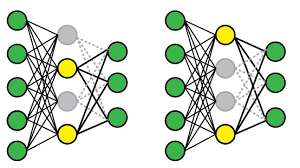
\includegraphics[scale=0.8]{images/dropout}
\caption{Neuronok véletlenszerű deaktiválása}
\label{fig:dropout}
\end{figure} 

\subsection{A háló tanítása}

Ez a neurális hálózatok használatának egyik lényeges pontja. Sok kérdés merülhet fel a megfelelő tanítási algoritmus kiválasztása közben.
\begin{itemize}
\item Hogyan ismerik az első konvolúciós rétegben lévő szűrők az élek és görbék keresését?
\item Hogyan ismeri fel a teljesen összekapcsolt réteg a jellemzőket?
\item Hogyan ismerik a szűrők az egyes rétegekben milyen értékeket kapnak?
\end{itemize}
A számítógép képes beállítani a szűrő értékeit (vagy súlyait) a backpropagation-nek nevezett eljárással.

A backpropagation négy különböző szakaszra osztható \cite{ABeginne32}:
\begin{itemize}
\item előre terjesztés (forward pass),
\item veszteség számítás (loss function),
\item hiba visszaterjesztés (backward pass),
\item súly frissítés (weight update).
\end{itemize}

Az előre terjesztés során egy kínai karakter képét (amelynek mérete például $48 \times 48$ pixel) továbbítunk az egész hálózaton. Az első leképzésnél, mivel minden súly és szűrőérték véletlenszerűen van inicializálva, így a kimenet is valószínűleg véletlenszerű lesz, ezért a hálózat nem add pontos osztályozást. A hálózat jelenlegi súlyaival nem tudja keresni az alacsony szintű jellemzőket, ilyenek például a stroke-ok. Emiatt tovább lépünk a veszteség számítás részre. Ne felejtsük el, hogy a tanító mintának van egy címkéje. A veszteségfüggvény többféle módon definiálható, de gyakori az \textit{MSE} (\textit{Mean Squared Error}, átlagos négyzetes hiba)
$$
E_{total} = \sum 1/2(target - output)^2.
$$ 

A \textit{target} egy vektor, aminek az értékei azt mutatják meg, hogy az adott minta a neurális háló döntése alapján mennyire illeszkedik a megfelelő karakterre. Ezt tipikusan úgy állítják össze, hogy a $0$ jelentse azt, hogy egyáltalán nem illeszkedik, az $1$ érték pedig, hogy a háló döntése alapján az a karakter teljesen illeszkedik.


A veszteség rendkívül magas az első képzésnél. Olyan pontra akarunk jutni, ahol az előre jelzett címke megegyezik a képzési címkével. Ahhoz, hogy odaérjünk, minimálisra csökkentjük a veszteségünket. Azt szeretnénk megtudni, hogy mely bemenetek/súlyok azok, amelyek leginkább hozzájárultak a hálózat veszteségéhez (vagy hibájához). Ezt az illeszkedést az alábbi módon határozhatjuk meg.

A négyzetes hibafüggvény szemléltetését láthatjuk \aref{fig:CNN_loss}. ábrán.

\begin{figure}[h]
\centering
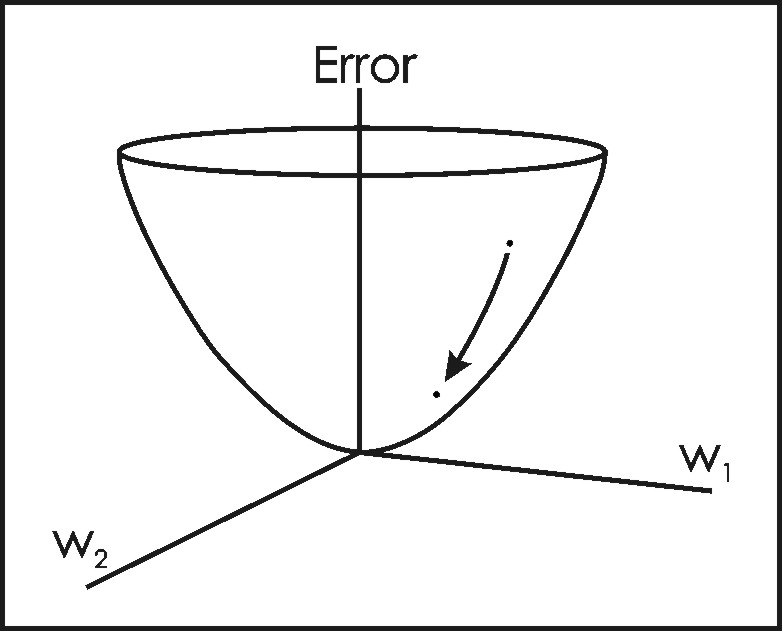
\includegraphics[scale=0.4]{images/CNN_loss}
\caption{A négyzetes hibafelület}
(forrás: \url{https://adeshpande3.github.io/A-Beginner%27s-Guide-To-Understanding-Convolutional-Neural-Networks/})
\label{fig:CNN_loss}
\end{figure}

A $dL/dW$ matematikai egyenlet írjuk fel a veszteség hozzájárulást. Következő lépés a hiba visszaterjesztés, amely meghatározza, hogy a súlyok milyen mértékben járultak hozzá a veszteséghez és megtalálják azokat a módokat, amelyekkel a károk csökkenthetők. Miután kiszámítjuk ezt a származékot, akkor megyünk az utolsó lépéshez, amely a súlyok frissítése. Itt vesszük az összes súlyt és szűröt és frissítjük őket úgy, hogy a gradiens ellenkező irányba változzon. Ekkor
$$
w = w_i - \eta \dfrac{dL}{dW},
$$
ahol $w$ a súly, a $w_i$ a kezdeti súly, az $\eta$ pedig a tanulási tényező.

A tanulási tényező egy olyan paraméter, amelyet a programozó választ. A magas tanulási arány azt jelenti, hogy nagyobb súlycsökkenést kell végrehajtani a súlycsökkentésekben, így kevesebb időre lehet szükség ahhoz, hogy a modell konvergáljon az optimális súlycsoporton. Azonban a túl magas tanulási arány olyan túl nagy ugrásokhoz vezethet, amelyek nem elég pontosak ahhoz, hogy elérjék az optimális pontot. Ennek egy szemléltetését láthatjuk \aref{fig:CNN_learning_rate}. ábrán.

\begin{figure}[h]
\centering
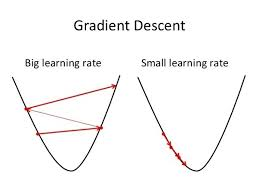
\includegraphics[scale=0.8]{images/CNN_learning_rate}
\caption{Magas és alacsony tanulási tényezők hatása}
(forrás: \url{https://adeshpande3.github.io/A-Beginner%27s-Guide-To-Understanding-Convolutional-Neural-Networks/})
\label{fig:CNN_learning_rate}
\end{figure}

Az előre terjesztés, a veszteség számítás, a visszaterjesztés és a paraméterfrissítés folyamata egy képzési iteráció. A program megismételi ezt a folyamatot egy rögzített számú iterációra. Miután befejezte a paraméter frissítést az utolsó képzésnél, remélhetőleg a hálózat megfelelően működik.

\subsection{Tesztelés}

Végül megnézzük, hogy működik-e a hálózat vagy sem. Különböző (még nem látott) képeket továbbíthatunk a CNN-en keresztül. Összehasonlítjuk a kimeneteket a címkékkel és megnézzük a hibát. Ha alacsony hibát kapunk a hálózat jól dolgozott.

\subsection{Transfer learning}

A konvolúciós hálózatok betanításához nagyszámú mintára és nagy teljesítményű számítógépekre van szükség. Amennyiben nem áll rendelkezésünkre nagyjából egymillió képkockából álló tanító adathalmaz, akkor kis számú mintáról beszélünk. Ha nincs lehetőségünk vagy erőforrásunk nagy adathalmazzal tanítani, akkor is megvalósíthatjuk a kívánt leképezést. A transfer learning (tanulás átadása) módszer segítségével egy előre betanított hálózatot veszünk alapul és annak utolsó pár rétegét lecserélve végezzük a tanítást. Ilyenkor a megmaradt rétegek betanított tulajdonság érzékelő funkciója segítségével a lecserélt rétegek által megvalósítandó leképezés könnyebbé vállhat. A konvolúciós neurális hálózatok tanítása esetében ez egy gyakori eljárás. Az interneten számos előre betanított hálózat található.

\Chapter{Tervezés és implementáció}

% TODO: Keras áttekintése.

% TODO: Szakaszonként bemutatni a jellemző kinyerés implementációját.

% TODO: Részletesen, osztálydiagrammal bemutatni a konvolúciós hálós osztályozáshoz készített program szerkezetét.

\Chapter{Validáció}

% TODO: Minél több konkrét példával, és számszerű eredménnyel szemléltetni a program működését és hatékonyságát!

\section{Adathalmaz}

A kínai karaktereket különböző kategóriákba is besorolhatjuk az előállításuk szerint.
\begin{itemize}
\item \textit{Nyomtatott}: A kijelzőkön megjelenített karakterek. Szélességét és magasságát pixelben adjuk meg. A felbontás növelése minőség növekedést eredményez, de a felismerés ideje nő. Több mint 100 betűtípus létezik.
\item \textit{Kézzel írt}: A betűtípus íronként változó. Léteznek nagy adathalmazok, ami segíti a gépi tanulást a kínai karakter felismerés során.
\item \textit{Generált}: Ebben az esetben egy modellt kell létrehozni, ami szerint generálunk. Az alapvonások elhelyezkedésének szabályait figyelembe véve lehetőségünk van bizonyos karakterek generálására.

Grafika szempontjából két csoportra gondolhatunk generálás során.
	\begin{itemize}
	\item Raszteres: Minden egyes képkockának megvan a maga színértéke, így áll össze a kép. Ebben az esetben a számítás igény magas (a sok képkocka sok számítást eredményez).
	\item Vektoros: Gyakorlatilag matematikai képletekkel rajzolunk. Egy egyenes (vektor) pontos meghatározásához három adat szükséges: kiindulópont, végpont koordinátái és a vonalvastagság.
	\end{itemize}
\end{itemize}

A generált adathalmazokat használata elönyös, hiszen nincs hozzáférési kötöttség az adatokhoz. Továbbá rugalmas, hiszen a modell változtatásával könnyedén lehet különböző karaktereket létrehozni (akár nem látottakat is). A minták generálása során vektoros grafikát használtam.

\subsection{A mintaadatok előkészítése a tanításhoz}

A tanító mintáknak különböznie kell a tesztelési mintáktól. A tanítási mintahalmazra a hálózat pontossága magasabb, hiszen a tesztelési pontokat nem ismeri.

Az arányok megválasztásánál gyakori a 80/20 (tanító/tesztelő) arány. Az én esetemben 4GB tanító 1GB tesztelő adathalmazt használok.

Az offline adatokkal végzem el a tanítást. \Aref{fig:offline_dataset}. ábrán láthatunk példát a kínai karakterekre.

\begin{figure}[h]
	\centering
	
\includegraphics[scale=2.0]{images/offline_dataset}
	\caption{Offline adatbázis példa}
	\label{fig:offline_dataset}
\end{figure} 

Az adathalmaz bejárása előtt azokat érdemes össze keverni véletlenszerűen. Ennek eredménye, hogy a hálózat minden egyes futtatás során egy picivel máshogy fog tanulni. A különbözöségek elkerülésére lehet használni egy úgynevezett \textit{seed}-et, aminek rögzítésekor megegyező módon keveri össze az adatokat. Ehhez a Python \texttt{random} modulja egyszerű megoldást biztosít.
\begin{python}
random.shuffle(self.image_names)
\end{python}

A keverés mellet véletlenszerű zajokat is hozzáadhatunk a képekhez (vágás, forgatás, elmosás). A zaj hozzáadáshoz a \texttt{imgaug} csomag rendkivül hasznos.

\begin{python}
from imgaug import augmenters as iaa

seq = iaa.Sequential([
    iaa.Crop(px=(0, 16)), # vágás 
    iaa.Fliplr(0.5), # horizontális forgatás (50%-ba) 
    iaa.GaussianBlur(sigma=(0, 3.0)) # elmosás 0-3.0 szigma-val
])
\end{python}

A \texttt{imgaug} dokumentációjában részletesen ismertetésre kerülnek az argumentumok (Flipud, Affine, SimplexNoiseAlpha, Dropout, Grayscale, Scale).

\section{Mintaadatok beolvasása}

A tanítás elött be kell olvasni a kínai karaktereinket. Mind a tanító mind a tesztelő adathalmaznak ki kell nyerni a címkéjét, ami meghatároza, hogy a kép milyen karakter.

A különböző zajokkal ellátott képeket külön-külön be lehet tanítani a hálózattal. Ebben az esetben szét kell választani a képeket zajok szerint, majd azokat betanítani.

\newpage

\section{Tesztelés}

A tesztelés során megvizsgálom, hogy mennyire érzékenyek az adott zajok a hálózatra. A tanítás fázisnál figyelembe kell venni kell venni azt, hogy ha ugyanolyan zajjal tanítjuk be a  hálózatot akkor azt csak azt fogja jól felismerni. Előállhat az overfitting.

Felismerés zajok szerint:
\begin{itemize}
\item Zaj nélküli: A kép zajjal nincs terhelve. A felismerés ebben az esetben a legmagasabb a zaj nélküli mintákra (90+\%), viszont a zajosított képeket nehezen ismeri fel.\Aref{fig:original} ábrán látható az eredti kép.

\begin{figure}[h!]
	\centering
	
\includegraphics[scale=1.0]{images/original}
	\caption{Eredeti kép}
	\label{fig:original}
\end{figure}

\item Pontszerű: A tanítást pontszerű zajjal terhelt képekre végezzük el. A rendszer nehezebben ismeri fel az utóbbi mintákat (75-80\%) és a zajnélküli mintákat (90\% felettiről lecsökken 84\%-ra) is. A pontszerű zajok nem okoznak nagy problémát, hiszen a konvolúciós réteg az összevonó réteg megfelelő paraméterizálása megoldja a gondot. \Aref{fig:noise}. ábrán látható a zajosított kép.

\begin{figure}[h!]
	\centering
	
\includegraphics[scale=1.0]{images/noise}
	\caption{Pontszerű zaj}
	\label{fig:noise}
\end{figure}

\item Forgatás A tanítás elforgatott képekkel. A $\pm$5-20 fokos origó körüli forgatás kis mértékben változtatja meg a hálózat felismerését. A nagyobb forgatások nagyon megnehezítik a képek felismerését (zaj nélküli esetben 92\%-ról lecsökken 78\%-ra, pontszerű zaj esetében 80\%-ról 70\%-ra). Azzal magyarázható hogy a forgatás során az alapvonások helyzete, iránya, vektorai megváltoznak. \Aref{fig:rotated}. ábrán látható az elforgatott kép.

\begin{figure}[h!]
	\centering
	
\includegraphics[scale=1.0]{images/rotate}
	\caption{Elforgatott kép}
	\label{fig:rotated}
\end{figure}
\newpage

\item Elmosás: A tanítás homályos/elmosódott képekkel. Kis mértékben befolyásolja a hálózat felismerés aranyát. A hálózat jól alkalmazkodik a homályosított képhez. \Aref{fig:blur}. ábrán látható az elmosódott kép.

\begin{figure}[h!]
	\centering
	
\includegraphics[scale=1.0]{images/blur}
	\caption{Elmosódott kép}
	\label{fig:blur}
\end{figure}

\end{itemize}
\Chapter{Összegzés}

A dolgozatomban ismertetésre került a kínai karakterek felépítése, írási módjuk, bemutatva azok építőelemeit az alapvonásokat (\textit{strokes}). Ezt követően bemutattam a vonásrendek szabályait, amely hasznos az online karakterfelismerésnél.

Részletezésre került az optikai karakterfelismerés (OCR) müködése, annak részei. Mivel a probléma már rég óta közismert, ezért áttekintésre kerültek a manapság használt OCR-es megoldások, amelyek képesek felismerni a különböző betűtípusokkal nyomtatott kínai karaktereket.

A jellemző kinyerés fontos szakasz az osztályozás elött. A dimenziószám redukálása csökkenti a futási időt a későbbi szakaszokban. Ez lehetővé teszi a magasabb összetettségű algoritmusok használatát, több hiperparaméter keresését, vagy több értékelés elvégzését. A fontos jellemzők megtalálása kulcsfontosságú az osztályozás során.

A tématerület bemutatásához szükségesnek látszott a neurális hálózat alapvető elemeinek, tanítási és tesztelési módjának bemutatása. Ezt követően a képfelismeréshez leginkább ajánlott (az elérhető irodalmak alapján vélhetően a leghatékonyabb) konvolúciós neurális hálózatra (CNN) esett a választás. Az ezzel foglalkozó fejezet kifejti a CNN rétegeinek működését, továbbá bemutat egy aránylag aktuális kutatási eredményt, amely a felismerés pontosságát hasonlítja össze különböző hálózat architektúrák szerint.

A tervezés során bemutattam a \textit{Keras} könyvtárat. Eleinte bonyolultnak tűnő konvolúciós és hagyományos neurális hálózat könnyedén implementálható a \textit{Keras} segítségével. A megfelelő csomagok importálása után részleteztem a rétegek müködését. Egy egyszerű architektúrát építettem ki.

A validáció során betekintést nyerhetünk az eredmények ellenőrzéséhez összeállított adathalmazba, és hogy hogyan változik a hálózat osztályozási hatékonysága a bemeneti képek és a zajjal való terhelés hatására. Összességében tehát a generált, zajjal terhelt mintákkal történő tanítási módszer jól kombinálható a konvolúciós neurális háló alapú osztályozási módszerrel.

\pagebreak

\section*{Summary}

In this work, I have presented the structure and the drawing of the hand-written chinese characters. Its basic elements are called strokes. After, I have considered the rules of the stroke ordering which are very useful for online character recognition.

The \textit{Optical Character Recognition} has presented in details. The original problem is well-known from a long time. Therefore, I have reviewed the contemporary methods of these OCR solutions, which are able to recognize different kind of chinese fonts.

The feature extraction is an essential step of the character recognition process. By reducing the number of dimensions it can be achieved better calculation times. It makes available the usage of more complex algorithms, larger number of optimization parameters or larger count of evaluations. The determination of important features has a key role in the classification process.

It seems to be necessary to consider the basic theory of artificial neural networks. It consists the learning algorithm, the testing steps. Furthermore, I have checked the proposed algorithms of the image recognition methods according to the literature. As the result of this research, I have decided to use the \textit{Convolutional Neural Network}. I have describes its mechanisms in details in a chapter. It shows a relatively new results in this topic, which compares the accuracy of this solution and consider its network architecture.

I have used the \textit{Keras} software library. It seems to be complicated in the first time, but it makes easier the implementation of CNN networks. I have shown the details of the implementation and the layers of the networks. I have used an own, simple network architecture.

In the validation phase, we can show the checking of the results of this work. I showed the sample sets and the changing of the classification accuracy when we use additional noises. Summary, the learning method by generated noise can be combined well with the methods of convolutional neural network based classification process.
 

% % \Chapter{Irodalomjegyzék}
\begin{thebibliography}{9}
\addcontentsline{toc}{chapter}{Irodalomjegyzék}
% \addcontentsline{toc}{chapter}{Irodalomjegyzék}

% TODO: Pontosítani kell majd a hivatkozásokat, és formázni!

\bibitem{feldolgozasi_szintek}
\texttt{http://www.tankonyvtar.hu/hu/tartalom/tamop412A/2011-0063\_15\_gepi\_latas/ch02.html}

\bibitem{ccr}
Chinese Character Recognition in Diverse Fonts
\texttt{http://citeseerx.ist.psu.edu/viewdoc/download?doi=10.1.1.93.64\&rep=rep1\&type=pdf}

\bibliography{bibliography}
\bibliographystyle{ieee}


\end{thebibliography}
 % 2

\bibliographystyle{acm}
\bibliography{dolgozat}

\end{document}
